\documentclass[11pt,a4paper,]{article}
\usepackage{lmodern}

\usepackage{amssymb,amsmath}
\usepackage{ifxetex,ifluatex}
\usepackage{fixltx2e} % provides \textsubscript
\ifnum 0\ifxetex 1\fi\ifluatex 1\fi=0 % if pdftex
  \usepackage[T1]{fontenc}
  \usepackage[utf8]{inputenc}
\else % if luatex or xelatex
  \usepackage{unicode-math}
  \defaultfontfeatures{Ligatures=TeX,Scale=MatchLowercase}
\fi
% use upquote if available, for straight quotes in verbatim environments
\IfFileExists{upquote.sty}{\usepackage{upquote}}{}
% use microtype if available
\IfFileExists{microtype.sty}{%
\usepackage[]{microtype}
\UseMicrotypeSet[protrusion]{basicmath} % disable protrusion for tt fonts
}{}
\PassOptionsToPackage{hyphens}{url} % url is loaded by hyperref
\usepackage[unicode=true]{hyperref}
\hypersetup{
            pdftitle={Distribution of Job Postings Across Australia in 2018},
            pdfborder={0 0 0},
            breaklinks=true}
\urlstyle{same}  % don't use monospace font for urls
\usepackage{geometry}
\geometry{a4paper, centering, text={16cm,24cm}}
\usepackage[style=authoryear-comp,]{biblatex}
\addbibresource{references.bib}
\usepackage{longtable,booktabs}
% Fix footnotes in tables (requires footnote package)
\IfFileExists{footnote.sty}{\usepackage{footnote}\makesavenoteenv{long table}}{}
\usepackage{graphicx,grffile}
\makeatletter
\def\maxwidth{\ifdim\Gin@nat@width>\linewidth\linewidth\else\Gin@nat@width\fi}
\def\maxheight{\ifdim\Gin@nat@height>\textheight\textheight\else\Gin@nat@height\fi}
\makeatother
% Scale images if necessary, so that they will not overflow the page
% margins by default, and it is still possible to overwrite the defaults
% using explicit options in \includegraphics[width, height, ...]{}
\setkeys{Gin}{width=\maxwidth,height=\maxheight,keepaspectratio}
\IfFileExists{parskip.sty}{%
\usepackage{parskip}
}{% else
\setlength{\parindent}{0pt}
\setlength{\parskip}{6pt plus 2pt minus 1pt}
}
\setlength{\emergencystretch}{3em}  % prevent overfull lines
\providecommand{\tightlist}{%
  \setlength{\itemsep}{0pt}\setlength{\parskip}{0pt}}
\setcounter{secnumdepth}{5}

% set default figure placement to htbp
\makeatletter
\def\fps@figure{htbp}
\makeatother


\title{Distribution of Job Postings Across Australia in 2018}

%% MONASH STUFF

%% CAPTIONS
\RequirePackage{caption}
\DeclareCaptionStyle{italic}[justification=centering]
 {labelfont={bf},textfont={it},labelsep=colon}
\captionsetup[figure]{style=italic,format=hang,singlelinecheck=true}
\captionsetup[table]{style=italic,format=hang,singlelinecheck=true}


%% FONT
\RequirePackage{bera}
\RequirePackage[charter,expert,sfscaled]{mathdesign}
\RequirePackage{fontawesome}

%% HEADERS AND FOOTERS
\RequirePackage{fancyhdr}
\pagestyle{fancy}
\rfoot{\Large\sffamily\raisebox{-0.1cm}{\textbf{\thepage}}}
\makeatletter
\lhead{\textsf{\expandafter{\@title}}}
\makeatother
\rhead{}
\cfoot{}
\setlength{\headheight}{15pt}
\renewcommand{\headrulewidth}{0.4pt}
\renewcommand{\footrulewidth}{0.4pt}
\fancypagestyle{plain}{%
\fancyhf{} % clear all header and footer fields
\fancyfoot[C]{\sffamily\thepage} % except the center
\renewcommand{\headrulewidth}{0pt}
\renewcommand{\footrulewidth}{0pt}}

%% MATHS
\RequirePackage{bm,amsmath}
\allowdisplaybreaks

%% GRAPHICS
\RequirePackage{graphicx}
\setcounter{topnumber}{2}
\setcounter{bottomnumber}{2}
\setcounter{totalnumber}{4}
\renewcommand{\topfraction}{0.85}
\renewcommand{\bottomfraction}{0.85}
\renewcommand{\textfraction}{0.15}
\renewcommand{\floatpagefraction}{0.8}


%\RequirePackage[section]{placeins}

%% SECTION TITLES


%% SECTION TITLES
\RequirePackage[compact,sf,bf]{titlesec}
\titleformat*{\section}{\Large\sf\bfseries\color[rgb]{0.7,0,0}}
\titleformat*{\subsection}{\large\sf\bfseries\color[rgb]{0.7,0,0}}
\titleformat*{\subsubsection}{\sf\bfseries\color[rgb]{0.7,0,0}}
\titlespacing{\section}{0pt}{2ex}{.5ex}
\titlespacing{\subsection}{0pt}{1.5ex}{0ex}
\titlespacing{\subsubsection}{0pt}{.5ex}{0ex}


%% TITLE PAGE
\def\Date{\number\day}
\def\Month{\ifcase\month\or
 January\or February\or March\or April\or May\or June\or
 July\or August\or September\or October\or November\or December\fi}
\def\Year{\number\year}

%% LINE AND PAGE BREAKING
\sloppy
\clubpenalty = 10000
\widowpenalty = 10000
\brokenpenalty = 10000
\RequirePackage{microtype}

%% PARAGRAPH BREAKS
\setlength{\parskip}{1.4ex}
\setlength{\parindent}{0em}

%% HYPERLINKS
\RequirePackage{xcolor} % Needed for links
\definecolor{darkblue}{rgb}{0,0,.6}
\RequirePackage{url}

\makeatletter
\@ifpackageloaded{hyperref}{}{\RequirePackage{hyperref}}
\makeatother
\hypersetup{
     citecolor=0 0 0,
     breaklinks=true,
     bookmarksopen=true,
     bookmarksnumbered=true,
     linkcolor=darkblue,
     urlcolor=blue,
     citecolor=darkblue,
     colorlinks=true}

\usepackage[showonlyrefs]{mathtools}
\usepackage[no-weekday]{eukdate}

%% BIBLIOGRAPHY

\makeatletter
\@ifpackageloaded{biblatex}{}{\usepackage[style=authoryear-comp, backend=biber, natbib=true]{biblatex}}
\makeatother
\ExecuteBibliographyOptions{bibencoding=utf8,minnames=1,maxnames=3, maxbibnames=99,dashed=false,terseinits=true,giveninits=true,uniquename=false,uniquelist=false,doi=false, isbn=false,url=true,sortcites=false}

\DeclareFieldFormat{url}{\texttt{\url{#1}}}
\DeclareFieldFormat[article]{pages}{#1}
\DeclareFieldFormat[inproceedings]{pages}{\lowercase{pp.}#1}
\DeclareFieldFormat[incollection]{pages}{\lowercase{pp.}#1}
\DeclareFieldFormat[article]{volume}{\mkbibbold{#1}}
\DeclareFieldFormat[article]{number}{\mkbibparens{#1}}
\DeclareFieldFormat[article]{title}{\MakeCapital{#1}}
\DeclareFieldFormat[article]{url}{}
%\DeclareFieldFormat[book]{url}{}
%\DeclareFieldFormat[inbook]{url}{}
%\DeclareFieldFormat[incollection]{url}{}
%\DeclareFieldFormat[inproceedings]{url}{}
\DeclareFieldFormat[inproceedings]{title}{#1}
\DeclareFieldFormat{shorthandwidth}{#1}
%\DeclareFieldFormat{extrayear}{}
% No dot before number of articles
\usepackage{xpatch}
\xpatchbibmacro{volume+number+eid}{\setunit*{\adddot}}{}{}{}
% Remove In: for an article.
\renewbibmacro{in:}{%
  \ifentrytype{article}{}{%
  \printtext{\bibstring{in}\intitlepunct}}}

\AtEveryBibitem{\clearfield{month}}
\AtEveryCitekey{\clearfield{month}}

\makeatletter
\DeclareDelimFormat[cbx@textcite]{nameyeardelim}{\addspace}
\makeatother

\author{\sf\Large\textbf{Mr. Justin Thomas}\\ {\sf\large Master of Business Analytics\\[0.5cm]} \sf\Large\textbf{Miss Peimin Lin}\\ {\sf\large Master of Business Analytics\\[0.5cm]} \sf\Large\textbf{Miss Hai Hanh Ngo}\\ {\sf\large Master of Business Analytics\\[0.5cm]} \sf\Large\textbf{Miss Dewi Lestari Amaliah}\\ {\sf\large Master of Business Analytics\\[0.5cm]}}

\date{\sf\Date~\Month~\Year}
\makeatletter
\lfoot{\sf Thomas, Lin, Ngo, Amaliah: \@date}
\makeatother


%%%% PAGE STYLE FOR FRONT PAGE OF REPORTS

\makeatletter
\def\organization#1{\gdef\@organization{#1}}
\def\telephone#1{\gdef\@telephone{#1}}
\def\email#1{\gdef\@email{#1}}
\makeatother
  \organization{Monash University}

  \def\name{Department of\newline Econometrics \&\newline Business Statistics}

  \telephone{(03) 9905 2478}

  \email{BusEco-Econometrics@monash.edu}

\def\webaddress{\url{http://buseco.monash.edu/ebs/consulting/}}
\def\abn{12 377 614 012}
\def\logo{
\includegraphics[width=6cm]{MBSportrait}}
\def\extraspace{\vspace*{1.6cm}}
\makeatletter
\def\contactdetails{\faicon{phone} & \@telephone \\
                    \faicon{envelope} & \@email}
\makeatother

%%%% FRONT PAGE OF REPORTS

\def\reporttype{Report for}

\long\def\front#1#2#3{
\newpage
\begin{singlespacing}
\thispagestyle{empty}
\vspace*{-1.4cm}
\hspace*{-1.4cm}
\hbox to 16cm{
  \hbox to 6.5cm{\vbox to 14cm{\vbox to 25cm{
    \logo
    \vfill
    \parbox{6.3cm}{\raggedright
      \sf\color[rgb]{0.00,0.00,0.70}
      {\large\textbf{\name}}\par
      \vspace{.7cm}
      \tabcolsep=0.12cm\sf\small
      \begin{tabular}{@{}ll@{}}\contactdetails
      \end{tabular}
      \vspace*{0.3cm}\par
      ABN: \abn\par
    }
  }\vss}\hss}
  \hspace*{0.2cm}
  \hbox to 1cm{\vbox to 14cm{\rule{1pt}{26.8cm}\vss}\hss\hfill}
  \hbox to 10cm{\vbox to 14cm{\vbox to 25cm{
      \vspace*{3cm}\sf\raggedright
      \parbox{11cm}{\sf\raggedright\baselineskip=1.2cm
         \fontsize{24.88}{30}\color[rgb]{0.70,0.00,0.00}\sf\textbf{#1}}
      \par
      \vfill
      \large
      \vbox{\parskip=0.8cm #2}\par
      \vspace*{2cm}\par
      \reporttype\\[0.3cm]
      \hbox{#3}%\\[2cm]\
      \vspace*{1cm}
      {\large\sf\textbf{\Date~\Month~\Year}}
   }\vss}
  }}
\end{singlespacing}
\newpage
}

\makeatletter
\def\titlepage{\front{\expandafter{\@title}}{\@author}{\@organization}}
\makeatother

\usepackage{setspace}
\setstretch{1.5}

%% Any special functions or other packages can be loaded here.


\begin{document}
\titlepage

{
\setcounter{tocdepth}{2}
\tableofcontents
}
\clearpage

\hypertarget{introduction}{%
\section{Introduction}\label{introduction}}

Job types, job locations, rising demand for certain job categories, these are just some of the aspects of job hunting that many working people around the world are intrigued by. In this report, you will find an in depth analysis into the distribution of job postings across Australia. The report will analyze 3 main sections of job distribution within Australia, broken down by:

\begin{enumerate}
\def\labelenumi{\arabic{enumi})}
\tightlist
\item
  The change in demand by job category
\item
  The change in demand for jobs by city
\item
  The change in demand by job type
\end{enumerate}

Our motivation to choose this as our research topic is prompted by being international students ourselves. As the unemployment rate in 2018 was at 5\%, which was the lowest level since May 2011 \textcite{unemployment}, this further intrigued our interest into understanding the job market in Australia. But we particularly wanted to know what the different jobs types and categories are in Australia, with an emphasis on how the job postings on the job employment website, SEEK, changed during 2018, particularly in the major cities.

\hypertarget{dataset-and-methodology}{%
\section{Dataset and Methodology}\label{dataset-and-methodology}}

\hypertarget{source-of-data}{%
\subsection{Source of Data}\label{source-of-data}}

To portray the change of job demand in Australia, we used an Australia job listing data downloaded from \href{https://www.kaggle.com/PromptCloudHQ/australian-job-listings-data-from-seek-job-board}{Kaggle} provided by \href{https://www.promptcloud.com}{PromptCloud}, a web-scraping company. Originally, this data was scraped from \href{https://www.seek.com.au}{Seek} job board. This dataset has a \href{https://creativecommons.org/licenses/by-sa/4.0/}{CC BY-SA 4.0} license, where people are free to share and adapt the data.

The other data source that was also utilised in this report is a cost of living dataset from \href{https://www.numbeo.com/cost-of-living/rankings.jsp?title=2018}{Numbeo}. It is a crowd-source global database with quality of life information. From the \href{https://www.numbeo.com/common/terms_of_use.jsp}{website's term of use}, it is mentioned that use, reuse, and distribution of Numbeo's content are allowed. Hence, the data can be used legally in this report. Furthermore, the table of Cost of Living Index by City 2018 was scraped using the rvest and polite packages.

\hypertarget{limitations-of-data}{%
\subsection{Limitations of Data}\label{limitations-of-data}}

\begin{itemize}
\tightlist
\item
  \textbf{Data collection method:} Even though the origin of data set was provided (obtained from Kaggle, collected by PromptCloud and scraped from Seek), it is hard to verify the credibility of the data set, whether the data was obtained in full and in completeness (with no observations being collected incorrectly). Instead the data was used as at the time of obtaining it from Kaggle.
\item
  \textbf{Sample size:} The collection period ran from 20 April 2018 to 26 October 2018 which accounted for 6 months of 2018. A sample set contained observations for less than one year period may hinder the ability to reflect seasonal cycle or pattern of the studied objects, which in turn may limit the explanatory power of the data set.
\item
  \textbf{Scope of discussion:} The data set was tidied, visualised and interpreted from the perspective of the individuals within this group. Thus, the opinions may be viewed, to some, as bias and incompleteness based on the personal experience and knowledge of the authors.
\end{itemize}

\hypertarget{methodology}{%
\subsection{Methodology}\label{methodology}}

\hypertarget{cleaning-the-dataset-and-inspecting-the-missing-values}{%
\subsubsection{Cleaning the dataset and inspecting the missing values}\label{cleaning-the-dataset-and-inspecting-the-missing-values}}

This is the data set pre - cleaning:

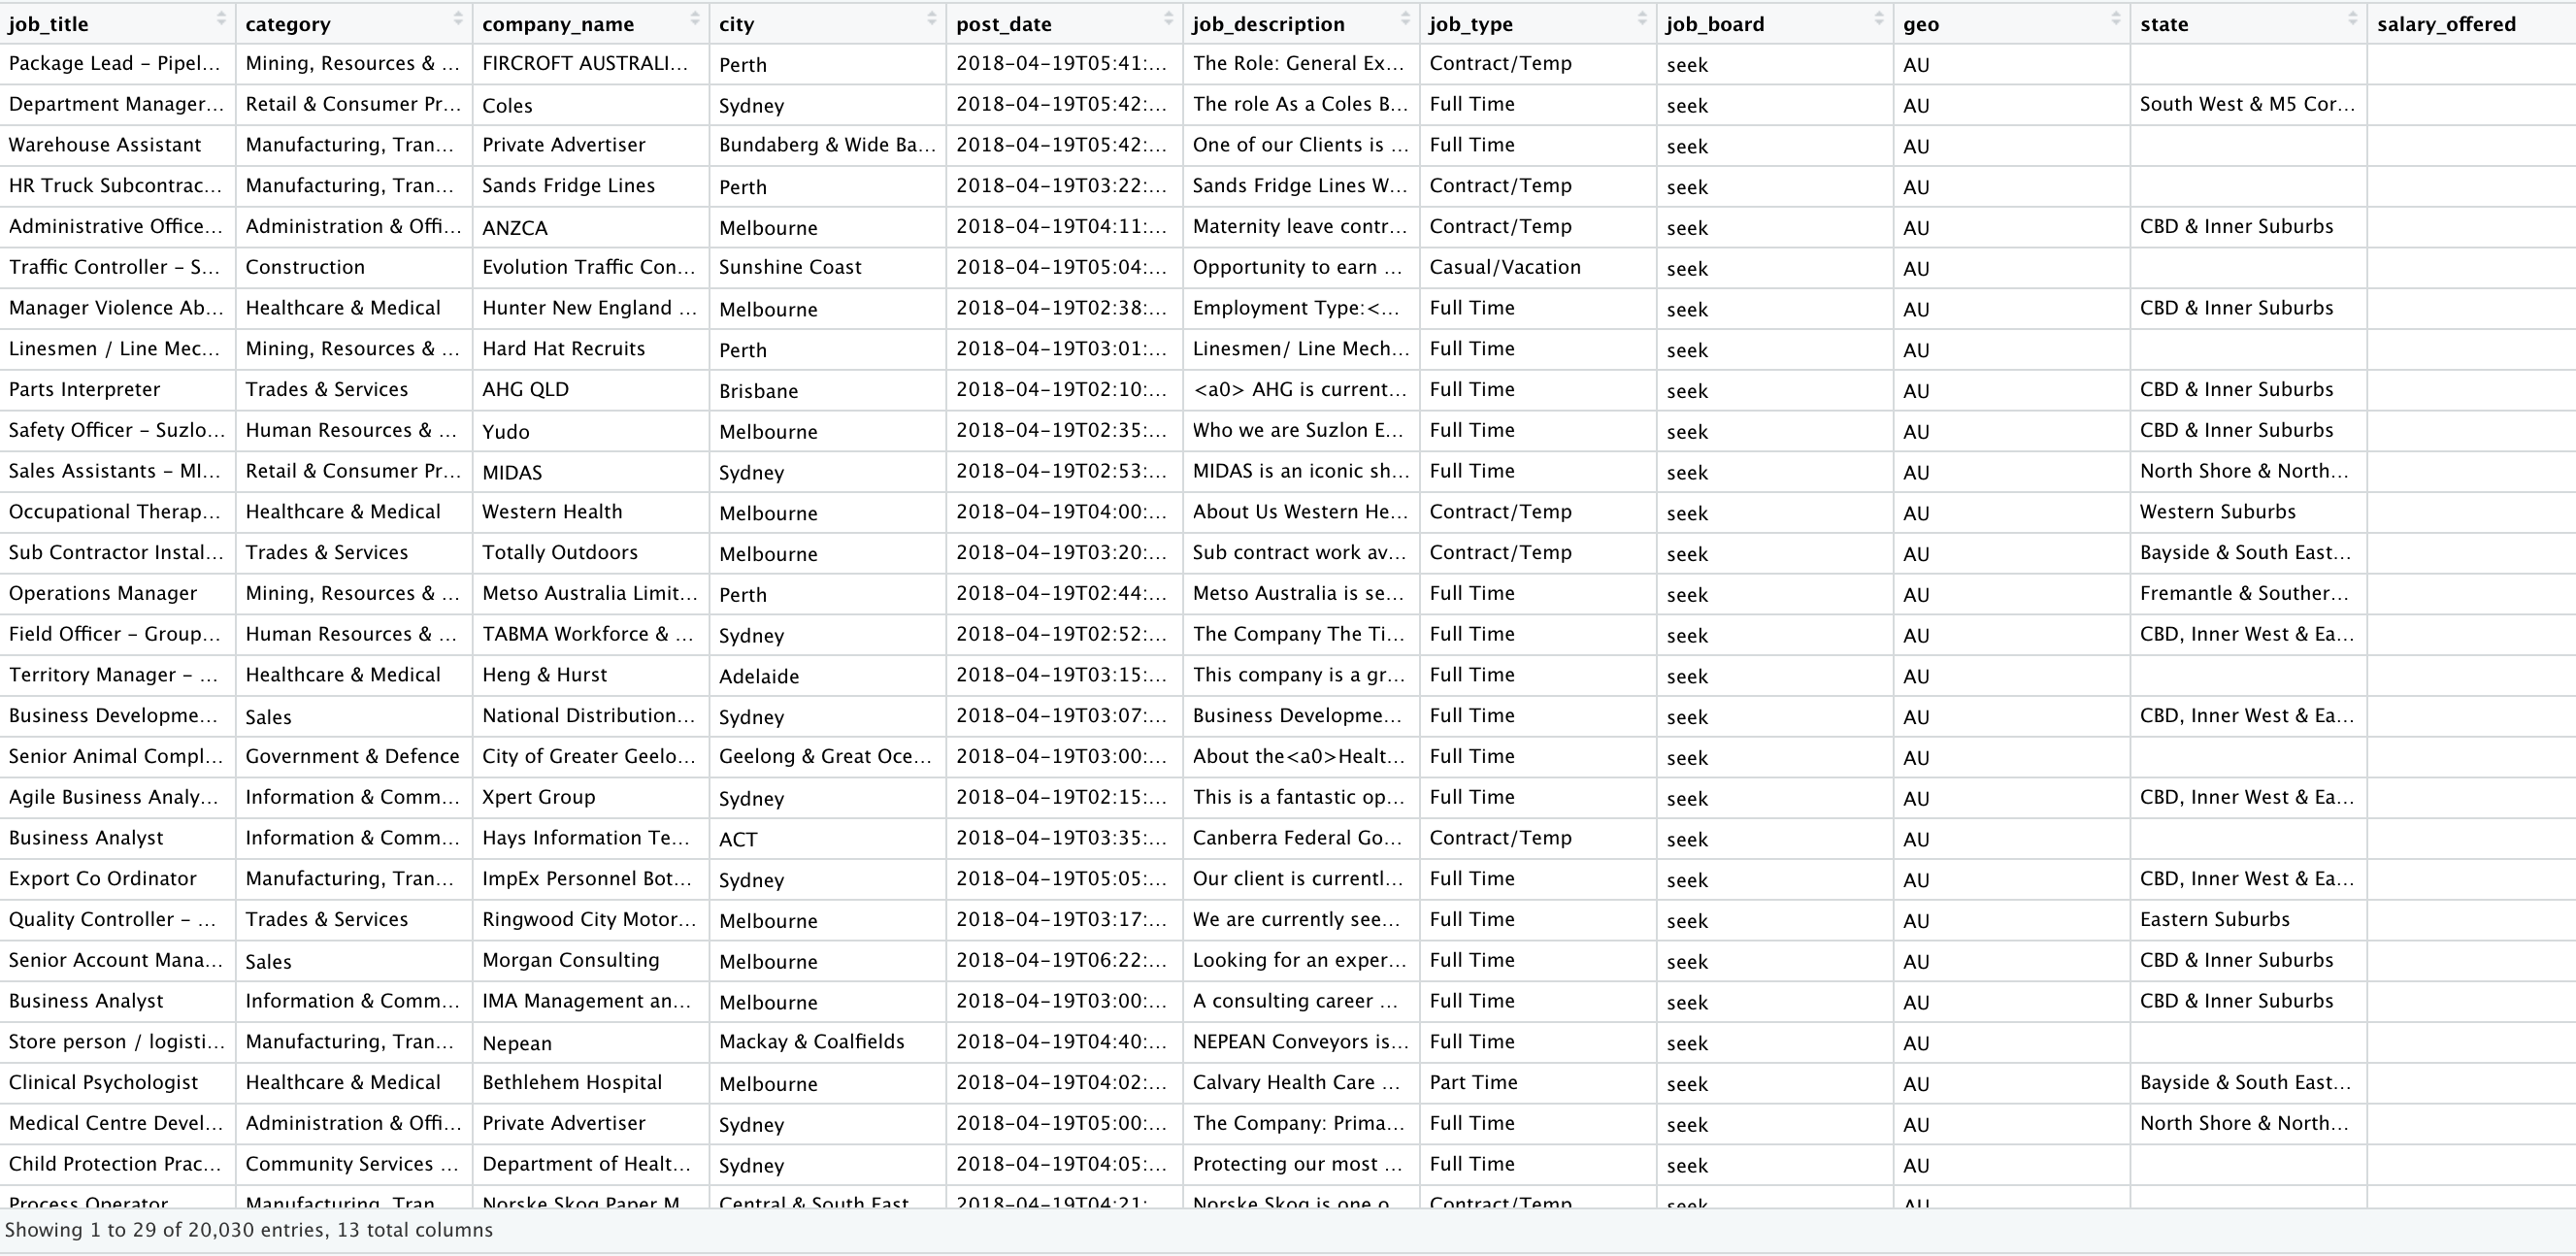
\includegraphics[width=1\linewidth]{C:/R/ETC5513/Assignment 4/JPHD-Assignment4/data/before}

There are things to note before we clean:

\begin{itemize}
\tightlist
\item
  \textbf{city:} there are observations that have multiple cities nested in one row.
\item
  \textbf{post\_date:} dates are coupled with time stamps, thus in character format not in date format.
\item
  \textbf{state:} nearly 30\% of state information are missing. Multiple name of states are nested in one row and are not in uniform format.
\item
  \textbf{geo:} contained both geographies of Australia and New Zealand.
\item
  \textbf{salary\_offered:} mostly absent.
\end{itemize}

In order for the data to be used, we needed to separate the nested column and observations, filter the data to include Australia only and filled out the state information, using the simplemap's list of cities and states in Australia (\textcite{simplemaps_2019}) to match with the cities in our data set.
This is the data set after we have done the cleaning, choosing only the variables needed for the analysis:

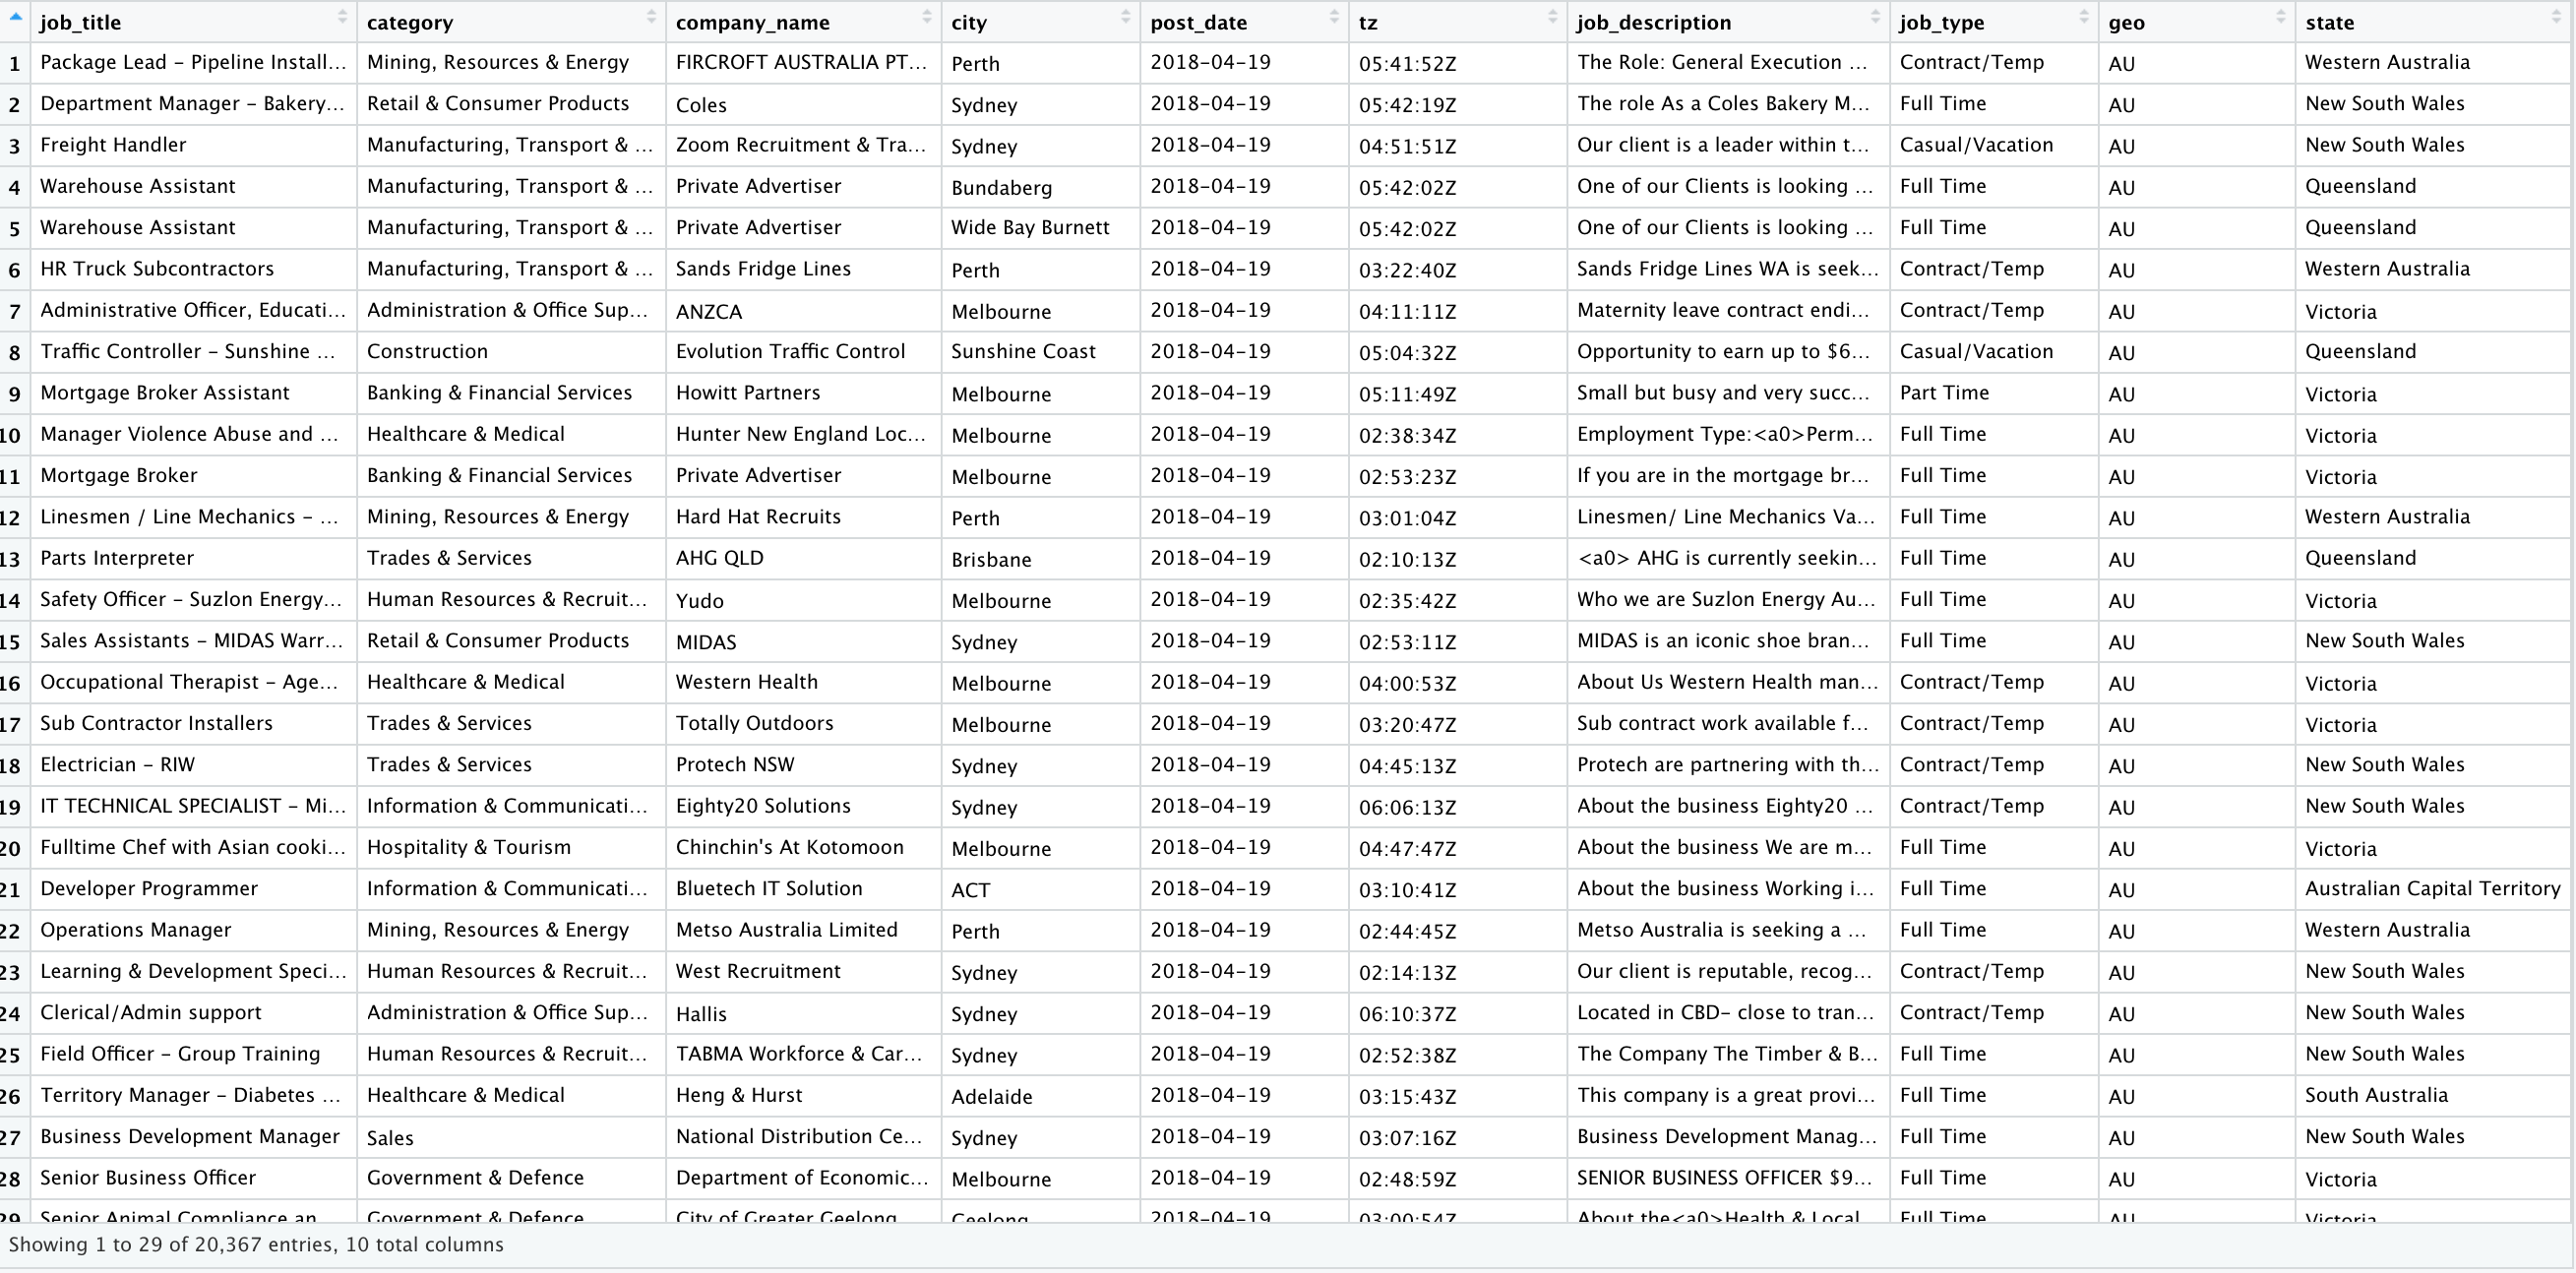
\includegraphics[width=1\linewidth]{C:/R/ETC5513/Assignment 4/JPHD-Assignment4/data/after}

After that, we inspected the missing values in the dataset.

\begin{figure}
\centering
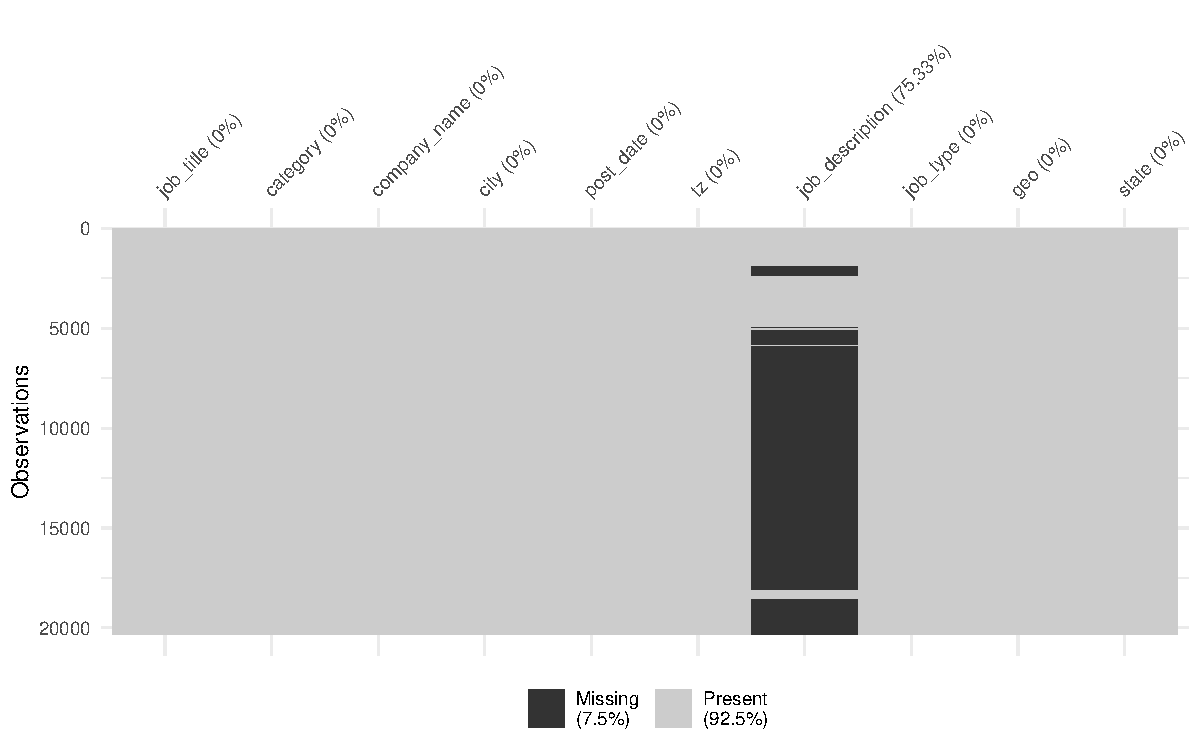
\includegraphics{Team_JHDP_Assignment4_files/figure-latex/missing-1.pdf}
\caption{\label{fig:missing}Missing values visualization after the cleaning}
\end{figure}

Figure \ref{fig:missing} showed that out of all variables chosen, job description is the only variable that had missing values and at a really high ratio, about 75.3\%, whereas other variables are fully present. However, job description is not of importance for this study, hence we can conclude that this data set requires no further cleaning and is ready for use.

\hypertarget{analyzing-the-data}{%
\subsection{Analyzing the data}\label{analyzing-the-data}}

An exploratory data analysis is performed to observe the change in job demand across Australia in 2018. We used a variety of plots using the functions in \texttt{ggplot2}. We also incorporated tables and did a correlation analysis using the Pearson coefficient correlation.

\hypertarget{analysis-and-conclusion}{%
\section{Analysis and Conclusion}\label{analysis-and-conclusion}}

\hypertarget{analyze-the-change-in-demand-by-job-category}{%
\subsection{Analyze the change in demand by job category}\label{analyze-the-change-in-demand-by-job-category}}

There are 30 job categories in this dataset and table \ref{tab:category} lists the number of jobs per category from April 2018 to November 2018. The job category of trades and services was the most popular job category in 2018 in Australia, followed by information and communications technology which saw the number of job postings as almost the same as the most popular job category. From the Labour Market Information Portal \autocite{welcome}, it is known that those two categories have been in short supply in the Australian labour market. Because of the small population and culture influence \autocite{burgess_2018}, automation cannot completely replace manual labour which is why the trade and services job category occupied the top spot.

\begin{table}

\caption{\label{tab:category} The number of jobs per category  }
\centering
\begin{tabular}[t]{l|r}
\hline
category & number\\
\hline
Self Employment & 16\\
\hline
CEO \& General Management & 82\\
\hline
Advertising, Arts \& Media & 104\\
\hline
Farming, Animals \& Conservation & 108\\
\hline
Science \& Technology & 108\\
\hline
Sport \& Recreation & 108\\
\hline
Insurance \& Superannuation & 133\\
\hline
Consulting \& Strategy & 139\\
\hline
Design \& Architecture & 247\\
\hline
Real Estate \& Property & 352\\
\hline
Legal & 385\\
\hline
Human Resources \& Recruitment & 448\\
\hline
Marketing \& Communications & 461\\
\hline
Banking \& Financial Services & 468\\
\hline
Mining, Resources \& Energy & 492\\
\hline
Community Services \& Development & 526\\
\hline
Call Centre \& Customer Service & 534\\
\hline
Engineering & 665\\
\hline
Education \& Training & 723\\
\hline
Retail \& Consumer Products & 766\\
\hline
Government \& Defence & 810\\
\hline
Construction & 894\\
\hline
Sales & 961\\
\hline
Accounting & 1084\\
\hline
Hospitality \& Tourism & 1141\\
\hline
Administration \& Office Support & 1250\\
\hline
Manufacturing, Transport \& Logistics & 1523\\
\hline
Healthcare \& Medical & 1535\\
\hline
Information \& Communication Technology & 1911\\
\hline
Trades \& Services & 2056\\
\hline
\end{tabular}
\end{table}

For a better timely observation across every month, figure \ref{fig:monthly} shows each job category's requirement change in different month which not only shows the shortage job, but also that the category is saturating. It is clear that there are some job categories that are in high demand in certain months of a year, for example, accounting has a high demand in June every year before the end of financial year. Additionally, there are other job categories that have seasonal requirements and result in a high demand during Christmas.

\begin{figure}
\centering
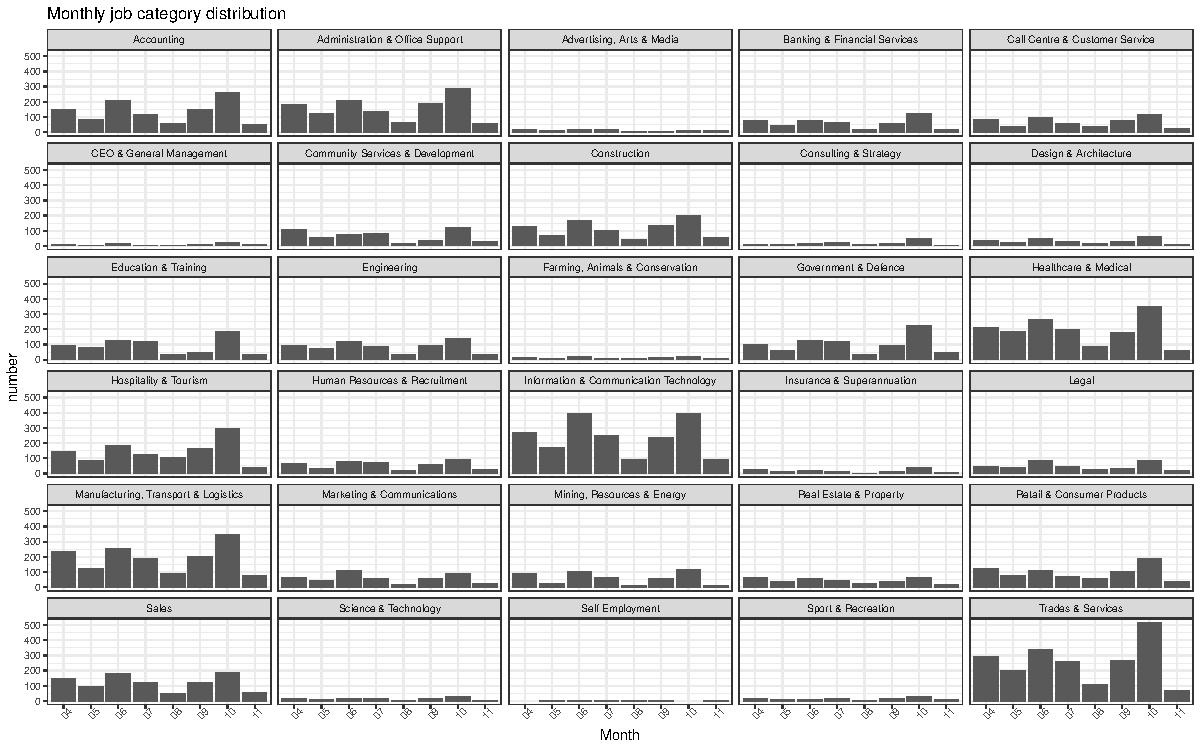
\includegraphics{Team_JHDP_Assignment4_files/figure-latex/monthly-1.pdf}
\caption{\label{fig:monthly}Monthly job category distribution}
\end{figure}

\begin{figure}
\centering
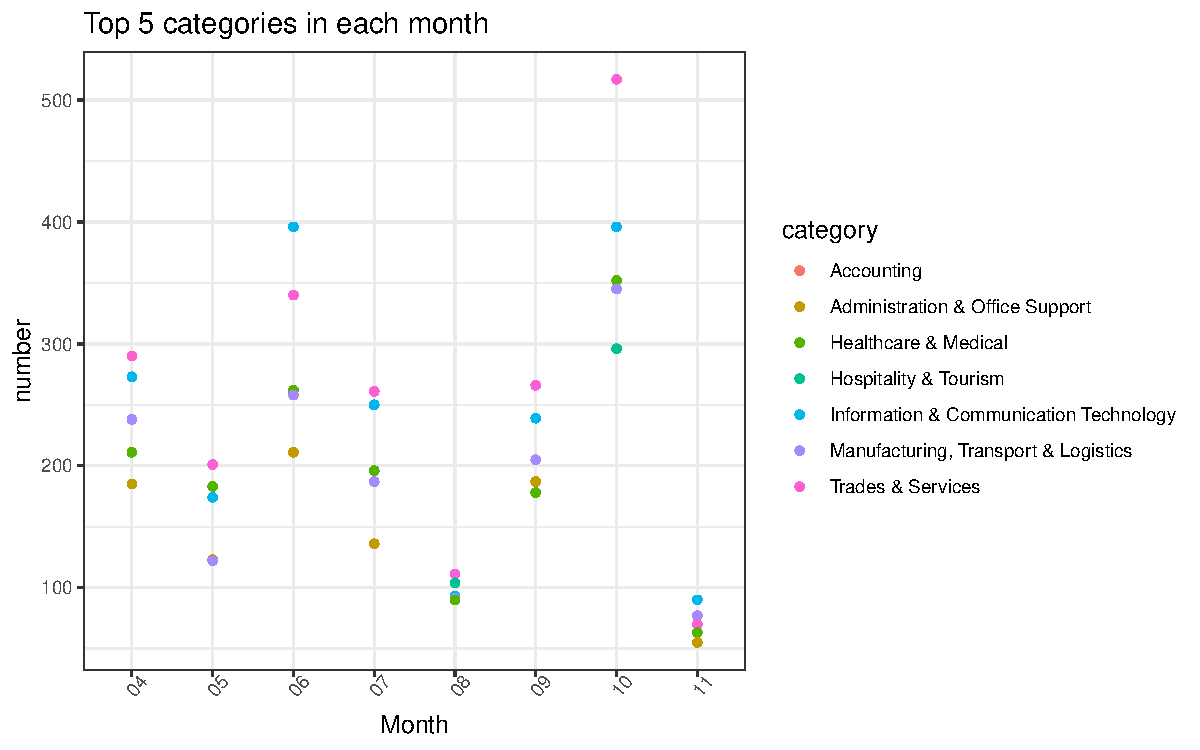
\includegraphics{Team_JHDP_Assignment4_files/figure-latex/number-1.pdf}
\caption{\label{fig:number}Top 5 category in each month}
\end{figure}

Meanwhile, figure \ref{fig:number} is a graph showing the top five job categories in each month. There are 7 categories that appears most frequently in the list such as accounting; administration and office support; healthcare and medical; hospitality and tourism; information and communication technology; manufacturing, transport and logistics; trade and services. In October, there were more vacancies and labour requirements than any other month. Forbes (\textcite{whitehead}) showed a statistics report indicating that most industries would figure out their labour requirements by September because the holiday season was coming up and the HR wants to finish their recruiting needs before the year-end. Thus, October became the busiest month for recruiting as the number of job postings increased. By the time November came around, the number of job postings in the whole labour market resulted in a sharp drop as the new round of hiring ended in October and hiring needs diminish before Christmas and New Year.

\hypertarget{analyze-the-change-in-job-demand-by-states}{%
\subsection{Analyze the change in job demand by states}\label{analyze-the-change-in-job-demand-by-states}}

\hypertarget{job-demand-in-states}{%
\subsubsection{Job demand in states}\label{job-demand-in-states}}

\begin{figure}

{\centering 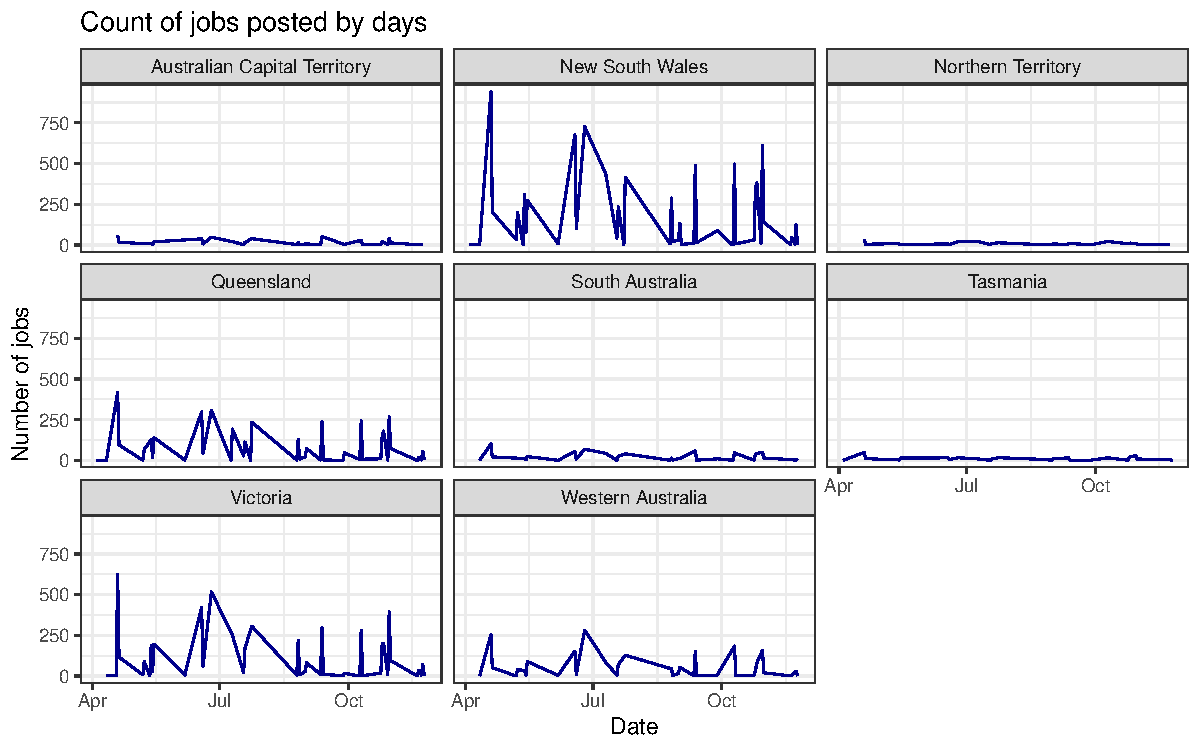
\includegraphics{Team_JHDP_Assignment4_files/figure-latex/state-demand-1} 

}

\caption{Daily job count by states}\label{fig:state-demand}
\end{figure}

Looking at figure \ref{fig:state-demand}, we can see that NSW, Victoria and Queensland lead the national job pool with the highest counts observed among all the states. The pattern of job posts appeared to look similar across the states with the highest peak in April, followed by two other minor peaks in July.

To have a better look at the states with lower job counts, which are Australia Capital Territory, Northern Territory, South Australia and Tasmania, we isolated them from the high-count states and looked at the change separately.

\begin{figure}
\centering
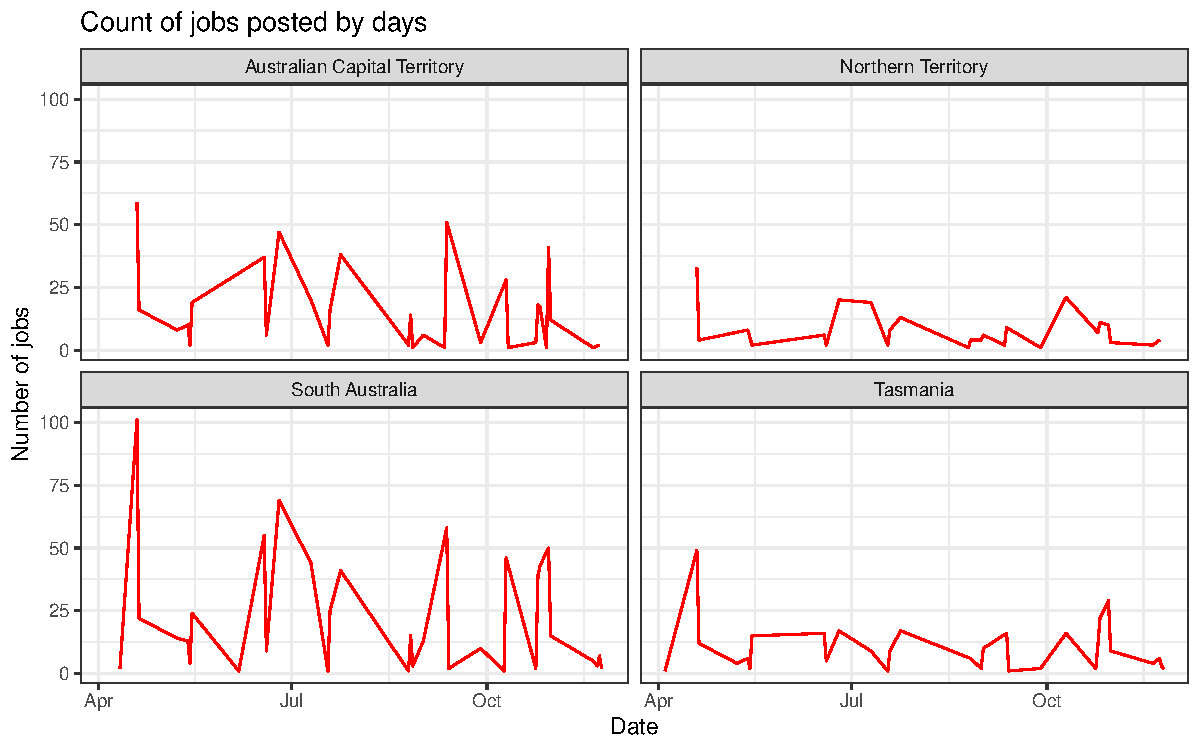
\includegraphics{Team_JHDP_Assignment4_files/figure-latex/low-demand-state-1.pdf}
\caption{\label{fig:low-demand-state}Daily job counts in ACT, NT, SA and TAS}
\end{figure}

Figure \ref{fig:low-demand-state} shows that the other four states had roughly the same pattern of job posts.

Normally, the job hunting season usually peaks around the beginning of the year, mostly in January as most companies have robust budgets for hiring and just came out of a holiday season in December. The same situation applies for job seekers as well as people who start to come back from the holiday, usually excited with a new year's resolution. Additionally, an annual bonus has been paid at the end of last year, making people more ready to change jobs starting from January \autocite{emswiler_2016}. This data set did not include data from January to March so we cannot verify the situation. However it would be safe to assume that this new year effect lasts further into April. Another peak is around July, which marks the start of new financial year for most companies, giving them higher budget for new hiring \autocite{emswiler_2016}.

Despite the similarity in seasonal pattern, the difference in job count was prominent across the states. Big states like NSW, Victoria and Queensland held the majority of opportunities, with the highest count reported at more than 7 times higher than the highest count in the low-demand states (NSW versus South Australia). Even though it is expected that big states would have more opportunities, the amount gap looked even more significant when presented visually.

\hypertarget{job-demand-and-living-cost}{%
\subsubsection{Job demand and living cost}\label{job-demand-and-living-cost}}

According to \textcite{davidlasswell}, when searching for a job, cost of living should be taken into account. It also relates to the question whether the salary of the job would be enough to cover the living cost in a particular city. Therefore, in this subsection, the living cost in some cities in Australia with relatively more job postings will be observed.

\begin{figure}
\centering
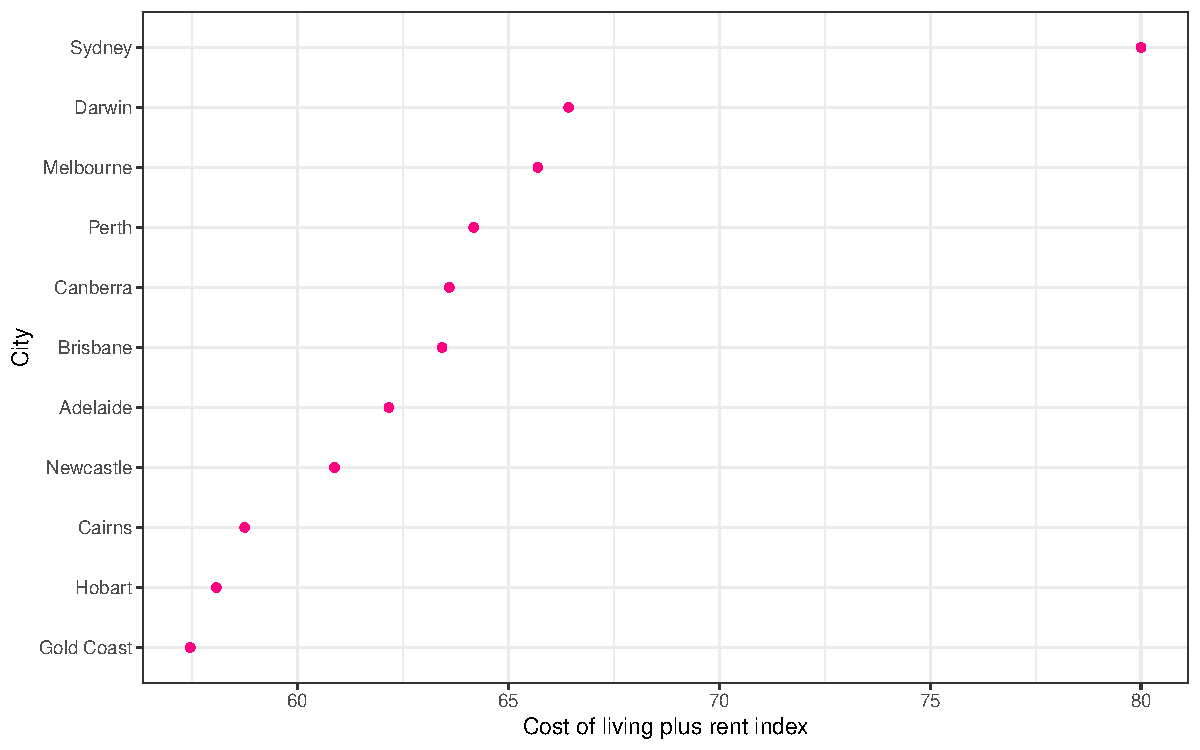
\includegraphics{Team_JHDP_Assignment4_files/figure-latex/livingcostplot-1.pdf}
\caption{\label{fig:livingcostplot}Living cost of 2018 by city}
\end{figure}

Figure \ref{fig:livingcostplot} shows that Sydney was found to be the city with the highest living cost, about 80. Whilst generally, the living cost index in most cities in Australia ranged betwen 60 to 68. The figure also conveys that Gold Coast was the city with the lowest living cost in Australia.
It is also interesting to observe whether there is a correlation between the living cost in those cities and the number of job postings there. Hence, the number of job postings in those cities will be examined first.

\begin{table}

\caption{\label{tab:jobcity}The number of job postings in some cities in Australia in 2018}
\centering
\begin{tabular}[t]{lr}
\toprule
City & Number of Job Postings\\
\midrule
Sydney & 5288\\
Melbourne & 4078\\
Brisbane & 1802\\
Perth & 1136\\
Adelaide & 542\\
\addlinespace
Canberra & 482\\
Newcastle & 352\\
Gold Coast & 297\\
Cairns & 148\\
Darwin & 110\\
\addlinespace
Hobart & 70\\
\bottomrule
\end{tabular}
\end{table}

Table \ref{tab:jobcity} conveys that Sydney is the city with most job postings. This city had more than 1000 jobs available between April to December 2018. Meanwhile, Hobart was found to be the city with the least job postings among others. The large number of job postings in Sydney is possibly due to the fact that Sydney was placed as the city with the highest productivity in Australia \autocite{pwcreport}.

\begin{figure}
\centering
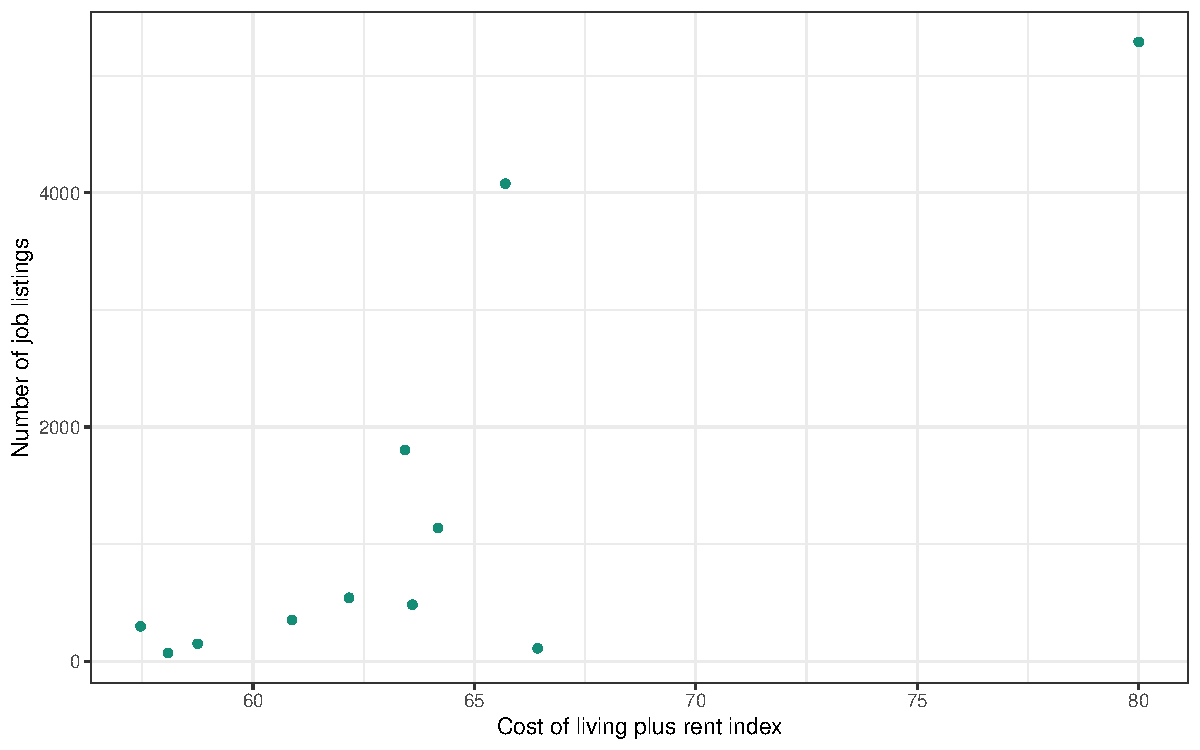
\includegraphics{Team_JHDP_Assignment4_files/figure-latex/corrplot-1.pdf}
\caption{\label{fig:corrplot}Cost of living plus rent index vs Number of job postings Scatter Plot}
\end{figure}

Figure \ref{fig:corrplot} suggests that there is a possible correlation between cost of living and the number of job postings in Australia. However, the pattern can not be really seen since the number of observations is too small. Therefore, the extension of analysis was performed by using the Pearson correlation coefficient. The finding is that there was a significantly positive (0.8211368) correlation between these two variables. This is inline with what \textcite{DePietro} stated that the increasing living cost is often associated with employment growth and income growth. Furthermore, larger cities tend to be perceived as expensive places to live \autocite{Weinstein}.

\hypertarget{analyze-the-change-in-demand-by-job-type}{%
\subsection{Analyze the change in demand by job type}\label{analyze-the-change-in-demand-by-job-type}}

In this section, our goal is to visualize the different types of jobs such as full-time, part-time, contract and casual jobs. The changes in demand to these job types will vastly differ across the months, but it will be interesting to see which job type increased in demand in 2018.

\hypertarget{number-of-jobs-posted-per-job-type}{%
\subsubsection{Number of jobs posted per job type}\label{number-of-jobs-posted-per-job-type}}

\begin{table}

\caption{\label{tab:job-type-counts}Number of jobs posted by job type}
\centering
\begin{tabular}[t]{l|r}
\hline
Job Type & Number of jobs posted\\
\hline
Casual/Vacation & 1459\\
\hline
Contract/Temp & 3685\\
\hline
Full Time & 13504\\
\hline
Part Time & 1382\\
\hline
\end{tabular}
\end{table}

\begin{figure}

{\centering 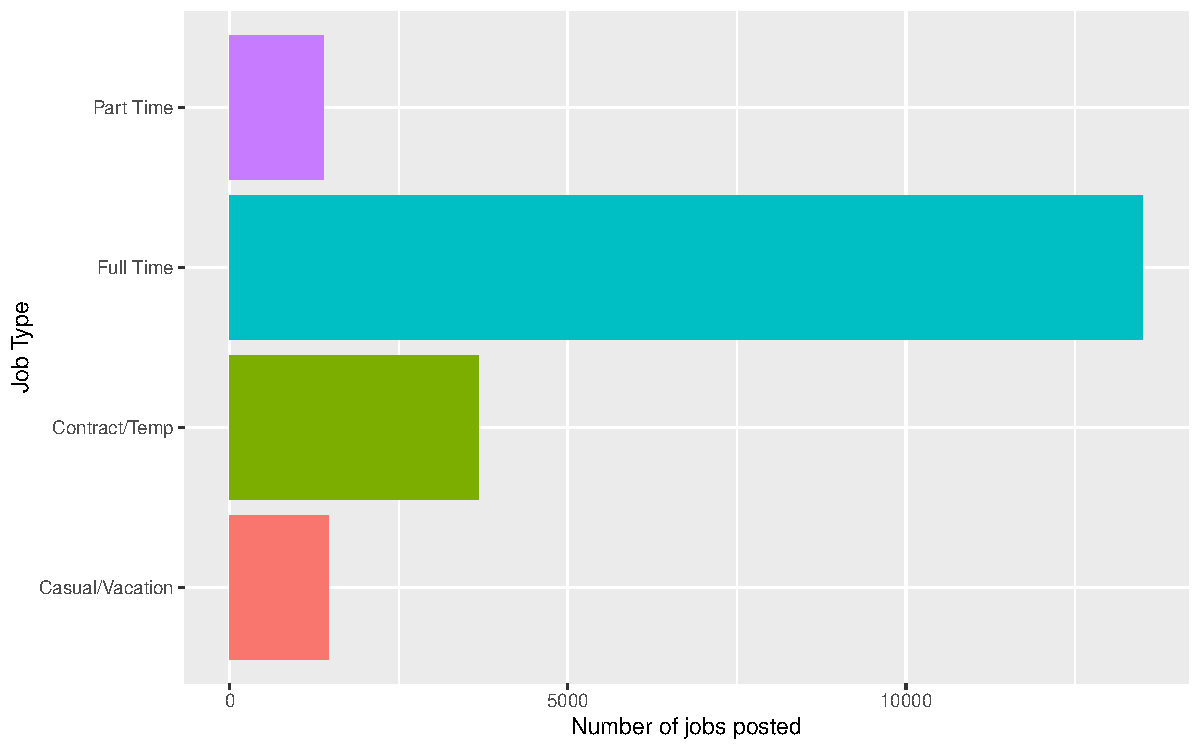
\includegraphics{Team_JHDP_Assignment4_files/figure-latex/job-types-1} 

}

\caption{Number of jobs for each job type}\label{fig:job-types}
\end{figure}

The different types of jobs being posted on SEEK are part time, full time, contract/temporary and casual/vacation. From Table \ref{tab:job-type-counts}, we can see that over 13500 jobs out of the roughly 20000 jobs posted are full-time jobs. It is easier to visualize just how common these types of jobs are in Figure \ref{fig:job-types}, and we can see how dominant the full-time jobs are being posted by companies. We can expect such a result as many companies want to employ fresh graduates from universities for an entry-level role. The number of new college graduates entering the workforce is always high enough for companies to post a lot of full-time jobs, which is why it is the most popular job type. Most of the full-time jobs are being generated in the healthcare and education sectors. Specifically, the National Disability Insurance Scheme (NDIS) and aged care services are seeing an increase in demand for these types of jobs. The NDIS expects an extra 80,000 full-time jobs by 2020 \textcite{aigroup}.

\hypertarget{fluctuations-in-job-posting-numbers-by-month}{%
\subsubsection{Fluctuations in job posting numbers by month}\label{fluctuations-in-job-posting-numbers-by-month}}

\begin{figure}

{\centering 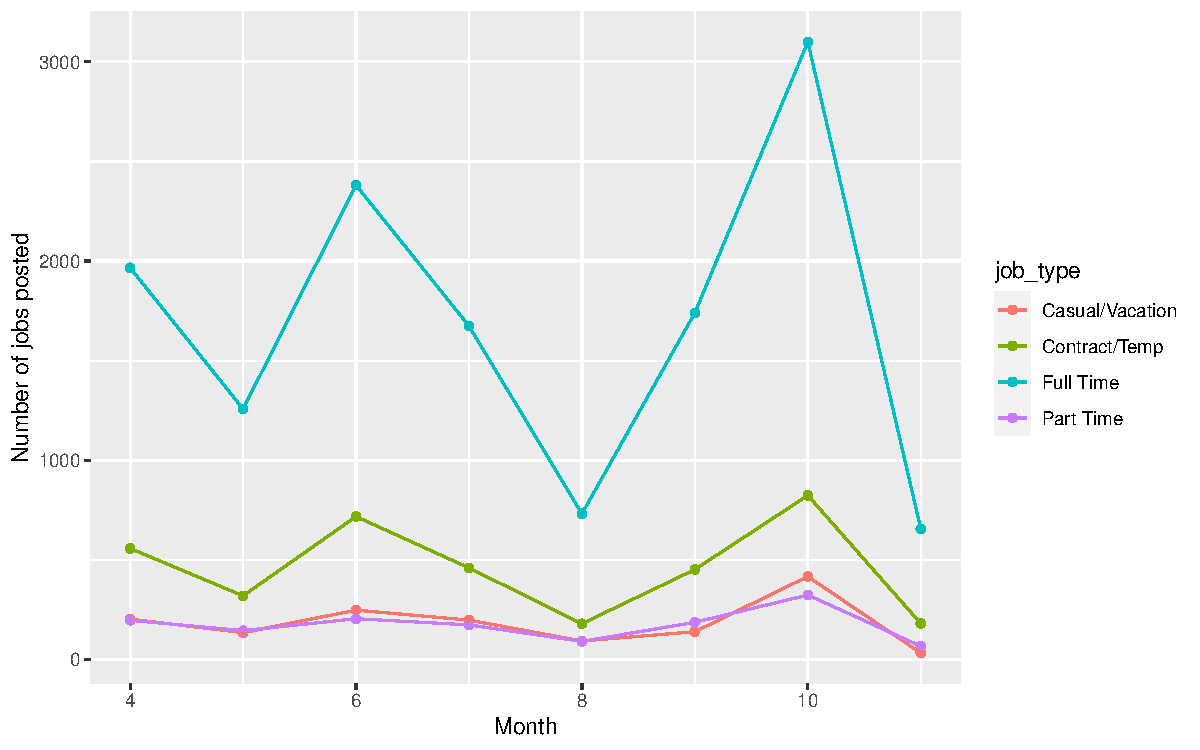
\includegraphics{Team_JHDP_Assignment4_files/figure-latex/job-count-fluctuations-1} 

}

\caption{Changes in job number postings by month}\label{fig:job-count-fluctuations}
\end{figure}

However, the fluctuations of these job types say more about what kind of jobs companies are willing to offer. For example, in Figure \ref{fig:job-count-fluctuations}, there is a large spike in full time jobs between August and October. The opposite is true when these jobs plummet down from 3100 posted jobs in October to around 700 jobs in November. Both part time and casual jobs stay relatively neutral and do not change as much throughout the months. Casual jobs have stayed the same since the past two decades, these jobs formed 20.6\% of the workforce in February 2018 compared to 20.1 \% in 1998. The reason for an uptick in the jobs posted for this category in October is because the largest proportion of people who take up casual jobs are aged 20-24, followed by people aged 15-19 \textcite{norman}. Thus around October, many of these people who are students are available to take on casual jobs as the summer break approaches. Interestingly, all the job types follow a similar pattern, reporting an increase in the number of jobs posted in June and October as these are the time periods for winter and summer break respectively.

\hypertarget{conclusion}{%
\section{Conclusion}\label{conclusion}}

The most common type of job posted on SEEK are full-time jobs. With an increasing number of graduates coming out of university, companies are finding ways to offer full-time roles to these graduates. Demand for full-time jobs is predicted to be highest in the healthcare industry with approximately 80,000 jobs needing to be filled by 2020. However, part-time and casual jobs for many different industries are still popular among individuals aged 15-19 and 20-24 even though the demand for these jobs have not changed much over the last 20 years.

In 2018, there are 30 job categories that appeared in the dataset, with trade and services and information technology ranking as the top categories for the labour market requirement. Meanwhile, we found that October was the busiest month for recruiting and some job categories have seasonal demand. Furthermore, the number of job postings in a city has a positive correlation with it's living cost. Sydney recorded the highest living cost index at 80 points, and had over 1000 jobs posted between April 2018 to December 2018. As such, states that have high living costs such as New South Wales, Victoria and Queensland holds a majority of the national job pool.

\hypertarget{acknowledgements}{%
\section{Acknowledgements}\label{acknowledgements}}

This report was written using R \autocite{Rcite}. The following R packages were used to produce this report: \texttt{tidyverse} \autocite{Rtidyverse}, \texttt{readr} \autocite{Readr}, \texttt{kableExtra} \autocite{Rkable}, \texttt{ggplot2} \autocite{Rggplot2}, \texttt{lubridate} \autocite{Rlubridate}, \texttt{tidyr} \autocite{Rtidyr}, \texttt{glue} \autocite{Rglue}, \texttt{naniar} \autocite{Rnaniar}, \texttt{polite} \autocite{Rpolite}, \texttt{rvest} \autocite{Rvest}, \texttt{xml2} \autocite{Rxml}, \texttt{forcats} \autocite{Rforcats}, \texttt{bookdown} \autocite{Rbookdown}, \texttt{MonashEBSTemplates} \autocite{monashebstemplate}, \texttt{knitr} \autocite{knitr}, \texttt{Rmarkdown} \autocite{rmarkdown}, \texttt{tinytex} \autocite{tinytex}.

\clearpage

\printbibliography[title=References]

\end{document}

